\documentclass[a4paper,12pt]{article} % добавить leqno в [] для нумерации слева
\usepackage[a4paper,top=1.3cm,bottom=2cm,left=1.5cm,right=1.5cm,marginparwidth=0.75cm]{geometry}
%%% Работа с русским языком
\usepackage{cmap}					% поиск в PDF
\usepackage{mathtext} 				% русские буквы в фомулах
\usepackage[T2A]{fontenc}			% кодировка
\usepackage[utf8]{inputenc}			% кодировка исходного текста
\usepackage[english,russian]{babel}	% локализация и переносы
\usepackage{multirow}

\usepackage{graphicx}

\usepackage{wrapfig}
\usepackage{tabularx}

\usepackage{hyperref}
\usepackage[rgb]{xcolor}
\hypersetup{
colorlinks=true,urlcolor=blue
}

%%% Дополнительная работа с математикой
\usepackage{amsmath,amsfonts,amssymb,amsthm,mathtools} % AMS
\usepackage{icomma} % "Умная" запятая: $0,2$ --- число, $0, 2$ --- перечисление

%% Номера формул
\mathtoolsset{showonlyrefs=true} % Показывать номера только у тех формул, на которые есть \eqref{} в тексте.

%% Шрифты
\usepackage{euscript}	 % Шрифт Евклид
\usepackage{mathrsfs} % Красивый матшрифт

%% Свои команды
\DeclareMathOperator{\sgn}{\mathop{sgn}}

%% Перенос знаков в формулах (по Львовскому)
\newcommand*{\hm}[1]{#1\nobreak\discretionary{}
{\hbox{$\mathsurround=0pt #1$}}{}}

%% Графики
\usepackage{tikz}
\usepackage{pgfplots}
\pgfplotsset{compat=1.9}

\date{\today}

\begin{document}

\begin{titlepage}
	\begin{center}
		{\large МОСКОВСКИЙ ФИЗИКО-ТЕХНИЧЕСКИЙ ИНСТИТУТ (НАЦИОНАЛЬНЫЙ ИССЛЕДОВАТЕЛЬСКИЙ УНИВЕРСИТЕТ)}
	\end{center}
	\begin{center}
		{\large Физтех-школа аэрокосмических технологий}
	\end{center}
	
	
	\vspace{4.5cm}
	{\huge
		\begin{center}
			{\bf Отчёт о выполнении лабораторной работы 1.4.1}\\
			Изучение экспериментальных погрешностей на примере физического маятника
		\end{center}
	}
	\vspace{1cm}
	\begin{center}
		{\large Соболевский Фёдор Александрович \\
			\vspace{0.2cm}
			Б03-109}
	\end{center}
	\vspace{8cm}
	\begin{center}
		Октябрь 2021
	\end{center}
\end{titlepage}

\section{Аннотация}

В работе на примере тонкого однородного металлического стержня, подвешиваемого в некоторой точке с помощью небольшой опорной призмы, исследованы закономерности колебаний физического маятника. Проверена справедливость формулы для периода колебаний физического маятника и закона Гюйгенса об обратимости
точек опоры и центра качания маятника. По экспериментальным значениям вычислено значение ускорения свободного падения. В ходе работы исследованы систематические и случайные погрешности прямых и косвенных измерений с целью оценить применимость данного метода определения ускорения свободного падения Земли и определить основные источники погрешностей в данном опыте.

\section{Теоретические сведения}

\begin{wrapfigure}{l}{0,3\textwidth}
	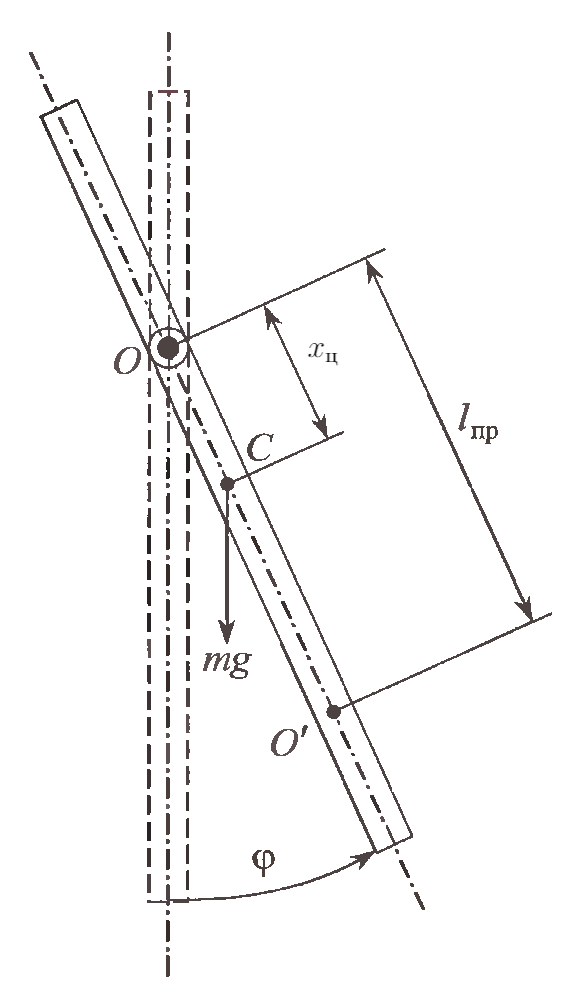
\includegraphics[width=0.91\linewidth]{ustanovka 1.4.1.png}
	\caption{Физический маятник}\label{risunok}
\end{wrapfigure}

Физическим маятником называют любое твердое тело, которое под действием силы тяжести может совершать свободные колебания вокруг неподвижной горизонтальной оси. Движение маятника описывается уравнением

\begin{equation}
J\frac{d^2\varphi}{dt^2}=M,
\label{osnova}
\end{equation}

\noindent где $ J $ -- момент инерции маятника, $ \varphi $ - угол между маятником и вертикальной осью, $ t $ - время, $ M $ - момент сил, действующих на маятник.

В данной работе в качестве физического маятника (рис.~ \ref{risunok}) используется однородный стальной стержень длиной $ l $. На стержне закрепляется опорная призма, острое ребро которой является осью качания маятника, а также дополнительный груз. Груз можно перемещать вдоль стержня, меняя таким образом положение центра масс системы. Пусть расстояние от точки опоры до центра масс маятника без груза равно $ x_\text{ц0} $. Тогда по теореме Гюйгенса-Штейнера момент инерции маятника без груза

\begin{equation}
J_0=\frac{ml^2}{12}+mx_\text{ц0}^2,
\label{momentOfInertia}
\end{equation}

\noindent где $ m $ -- масса маятника.В качестве подвижного груза в работе используется металлический цилиндр или «чечевица». Диаметр груза $ d_\text{г}$ ~6 см. Поскольку размер груза мал по сравнению с длиной стержня, его можно
считать закреплённой на стержне точечной массой. Обозначим за $ y $ расстояние от точки подвеса до центра масс груза, $ m_\text{г}$. Тогда момент
инерции маятника будет равен 

\begin{equation}
    J=J_0+m_\text{г}y^2,
\end{equation}

На практике величину $ y $ определять затруднительно, однако её можно вычислить через расстояние $ x_\text{ц} $ от точки опоры до центра масс всей системы и $ x_\text{ц0} $. Расстояние от точки подвеса до центра масс всей системы 

\begin{equation}
    x_\text{ц}=\frac{mx_\text{ц0}+m_\text{г}y}{M}
\end{equation}

\noindent где $ M $ - суммарная масса системы. Отсюда расстояние до центра масс груза равно

\begin{equation}
    y=\frac{Mx_\text{ц}-mx_\text{ц0}}{m_\text{г}}
    \label{counterweightCenter}
\end{equation}

Момент силы тяжести, действующий на маятник, 

\begin{equation}
M=-mga\sin\varphi.
\end{equation}

\noindent Если угол $ \varphi $ мал, то $ \sin\varphi\approx\varphi $, так что

\begin{equation}
M\approx-mga\varphi
\end{equation}

\noindent В исправной установке маятник совершает несколько сот колебаний без заметного затухания. Поэтому моментом силы трения в первом приближении можно пренебречь. Подставляя выражение для $ I $ и $ M $ в \eqref{osnova}, получим уравнение

\begin{equation}
\ddot{\varphi}+\omega^2\varphi=0,
\label{phi}
\end{equation}

\noindent где

\begin{equation}
\omega^2=\frac{Mgx_\text{ц}}{J_0+m_\text{г}y^2}.
\end{equation}

Тогда период колебаний равен

\begin{equation}\label{period}
T=\frac{2\pi}{\omega}=2\pi\sqrt{\frac{J_0+m_\text{г}y^2}{Mgx_\text{ц}}}
\end{equation}

Таким образом, период малых колебаний не зависит ни от начальной фазы, ни от амплитуды колебаний. Это утверждение (изохорность) справедливо для колебаний, подчиняющихся уравнению \eqref{phi}. Движение маятника описывается по этой формуле только для малых углов $ \varphi $.

\medskip

Величину

\begin{equation}\label{prLength}
l_\text{пр}=x_\text{ц0}+\frac{l^2}{12x_\text{ц0}}
\end{equation}

называют приведённой длиной математического маятника. Точку $ O' $ (см. рис. \ref{risunok}), отстоящую от точки опоры на расстояние $ l_\text{пр} $, называют центром качания физического маятника. С данными понятиями связана теорема Гюйгенса, которая утверждает, что точка опоры и центр качания маятника обратимы, т.е. при качании маятника вокруг  точки $ O' $ период будет таким же, как и при качании вокруг точки $ O $. 

Колебания можно считать гармоническими на определённом промежутке времени, если их затухание за этот промежуток мало. Затухание колебаний характеризует величина $ \gamma = -\frac{dA}{A}$ - декремент затухания, где $ A $ - амплитуда колебаний. Его можно найти из уравнения

\begin{equation}
    A=A_0e^{-\gamma t}
\label{decrement}
\end{equation}

Ещё одна характеристика колебательной системы - её добротность

\begin{equation}
    Q=\pi\frac{\tau_\text{зат}}{T}
\end{equation}
где $ \tau_\text{зат}=\frac{1}{\gamma}$ - время затухания колебаний в $ e $ раз.

\section{Оборудование и экспериментальные погрешности}

\textbf{Счётчик:} $ \Delta_c = 0,005 \text{ с}$\\
\textbf{Штангенциркуль:} $ \Delta_\text{шт} = 0,05 \text{ мм}$\\
\textbf{Весы:} $ \Delta_вес = 0,05 \text{ г}$ \\
Оценим максимальную точность измерений. Максимальные значения длины и массы, измеряемых в данном опыте, равны примерно 1 м и 400 г. Максимальная достижимая точность равна $ \epsilon = \sqrt{\epsilon_l^2+\epsilon_m^2} = \sqrt{(\frac{0,05 \text{ г}}{400 \text{ г}})^2+(\frac{0,05 \text{ мм}}{1000 \text{ мм}})^2}\approx 0,05\% $ Следовательно, для получения конечного результата с данной точностью следует измерять период с точностью не хуже $\approx 0,05\%$

\section{Результаты измерений и обработка данных}

\subsection{Измерение длин и масс, предварительный эксперимент}

\textbf{Длина стержня:} $ l = 1001,0 \text{ мм}$\\
\textbf{Масса стержня с призмой:} $ m = 1091,6 \text{ г}$\\
\textbf{Масса груза:} $ m_\text{г} = 372,5 \text{ г}$\\
\textbf{Масса стержня с грузом:} $ M = m + m_\text{г} = 1464,1 \text{ г}$\\
\textbf{Расстояние от оси качания до центра масс стержня без груза:} $ x_\text{ц0} = 283,2 \text{ мм}$\\
\textbf{Момент инерции стержня без груза:} $ J_0 = mx_\text{ц0}^2 = 0,1787 \text{кг} \cdot \text{м}^2$

Для проверки оборудования был проведён предварительный эксперимент без груза. Формула \eqref{momentOfInertia} приводится к виду

\begin{equation}
    T_0 = 2\pi\sqrt{\frac{\frac{l^2}{12}+x_\text{ц0}^2}{x_\text{ц0}g}}
    \label{prepPeriod}
\end{equation}

Период колебаний находится из полного времени измерения $t_\text{изм}$ и количества измерений $N_\text{изм}$ по формуле

\begin{equation}
     T = \frac{t_\text{изм}}{N_\text{изм}}
     \label{measurementPeriod}
\end{equation}

При $ N_\text{изм} = 20 $ $ t_\text{изм} = 30,49 \text{ c}$. Из \eqref{measurementPeriod} $ T_0 = 1,5245 \text{c}$ и по формуле \eqref{prepPeriod} найдено значение ускорения свободного падения

\begin{equation}
    g = 4\pi^2 \frac {\frac{l^2}{12} + x_\text{ц0}^2}{x_\text{ц0}T_0^2} = 9,8189 \text{ м/c}^2
\end{equation}

Полученное значение отличается от табличного ($ 9,8154 \text{ м/с}^2$) меньше, чем на 0,1\%, поэтому можно считать, что оборудование не создавало значительных ошибок при измерениях.

\subsection{Измерение периода колебаний маятника при разных положениях груза}

При закреплении груза в первом положении расстояние до центра масс системы оказалось равным $x_\text{ц1} = 369,7 \text{мм}$. По формуле \eqref{counterweightCenter} найдено значение $ y_1 = 623,2 \text{ мм}$. Для остальных измерений величина $ y $ определялась через смещение $ \Delta y $ относительно первого положения в сторону оси качания. 

Период колебаний измерен из времени $ t $ для $ N_\text{изм} = 20 $ колебаний для восьми разных положений груза. Для каждого опыта вычислено соответствующее значение ускорения свободного падения из формулы \eqref{period}:

\begin{equation}
    g = 4\pi^2 \frac{J_0 + m_\text{г}y^2}{Mx_\text{ц}T^2}
\end{equation}

Результаты измерений представлены в таблице \ref{tab1}.

\begin{table}[]
    \centering
    \begin{tabular}{c|c|c|c|c|c|c}
        № опыта & $ \Delta y $, мм & $ y $, мм & $ x_\text{ц} $, мм & $ t $, с & $ T $, с & $ g $, $ \text{м/с}^2 $ \\ \hline
        1 & 0 & 623,2 & 369,7 & 30,97 & 1,5485 & 9,836 \\
        2 & 30,0 & 593,2 & 357,9 & 30,63 & 1,5315 & 9,950 \\
        3 & 60,0 & 563,2 & 349,3 & 30,30 & 1,5150 & 9,984 \\
        4 & 90,0 & 533,2 & 345,8 & 30,00 & 1,5000 & 9,863 \\
        5 & 120,0 & 503,2 & 338,0 & 29,72 & 1,4860 & 9,863 \\
        6 & 150,0 & 473,2 & 330,4 & 29,45 & 1,4725 & 9,866 \\
        7 & 180,0 & 443,2 & 323,1 & 29,20 & 1,4600 & 9,861 \\
        8 & 210,0 & 413,2 & 316,0 & 28,96 & 1,4480 & 9,861 \\
    \end{tabular}
    \caption{Результаты измерения периода колебаний и ускорения свободного падения для разных положений груза}
    \label{tab1}
\end{table}

Методом непосредственного усреднения определено значение g

\begin{equation}
    \overline{g} = \frac{1}{N} \sum_{i=1}^{N} g_i = 9,8855 \text{ м/с}^2
\end{equation}

Случайная погрешность определения среднего при этом равна

\begin{equation}
    \sigma_{\overline{g}}^{\text{случ}} =\sqrt{\frac{1}{N(N-1)}\sum_{i=1}^{N}(g_i-\overline{g})^2} = 0,0184 \text{ м/с}^2
\end{equation}

Величина $ g $ находится из непосредственно измеряемых величин по формуле

\begin{equation}
    g = \frac{4\pi^2}{T^2} ( \frac{m_0l^2}{12Mx_\text{ц}} + \frac{mx_\text{ц0}^2}{Mx_\text{ц}} + \frac{Mx_\text{ц}}{m_\text{г}} + \frac{m_0^2x_\text{ц0}^2}{Mm_\text{г}x_\text{ц}} + \frac{2m_0x_\text{ц0}}{m_\text{г}} )
\end{equation}

Систематическая погрешность косвенных измерений измеряется по общей формуле

\begin{equation}
    \sigma_{f(x_1, x_2, x_3, ...) } = \sqrt{(\frac{df}{dx_1}\Delta x_1)^2 + (\frac{df}{dx_2}\Delta x_2)^2 +(\frac{df}{dx_3}\Delta x_3)^2 + ...}
\end{equation}

Отсюда вычислена систематическая погрешность косвенного измерения

\begin{equation}
    \sigma_{\overline{g}}^{\text{сист}} \approx 0,0193 \text{ м/с}^2
\end{equation}

Полная погрешность измерения составила 

\begin{equation}
     \sigma_{\overline{g}} = \sqrt{ (\sigma_{\overline{g}}^{\text{сист}})^2 +  (\sigma_{\overline{g}}^{\text{случ}})^2} \approx 0,0267 \text{ м/с}^2
\end{equation}

Далее величина g найдена по методу наименьших квадратов путём построения аппроксимируюшей прямой. С использованием формулы для периода физического маятника \eqref{period} получено следующее соотношение:

\begin{equation}
T^2x_\text{ц}=\frac{4\pi^2m_\text{г}}{Mg}y^2+\frac{4\pi^2J_0}{Mg}.
\end{equation}
Из этого соотношения видно, что $ T^2x_\text{ц} $ линейно зависит от $ y^2 $, поэтому это зависимость можно представить в виде

\begin{equation}
T^2x_\text{ц}=ky^2+b,
\end{equation}
где
\begin{equation}\label{koef}
k=\frac{4\pi^2m_\text{г}}{Mg} \text{ и }  b = \frac{4\pi^2J_0}{Mg}.
\end{equation}

Найдём эти коэффициента. Для удобства все необходимые данные представлены в таблице \ref{tab3}.

\begin{table}[h!]
	\begin{tabular}{|c|c|c|c|c|c|c|c|c|} \hline
		№ опыта  & 1 & 2 & 3 & 4 & 5 & 6 & 7 & 8  \\ \hline
		$ y $, м & 0,6232 & 0,5932 & 0,5632 & 0,5332 & 0,5032 & 0,4732 & 0,4432 & 0,4132 \\ \hline
		$ y^2 $, $ \text{м}^2 $  & 0,3883 & 0,3518 & 0,3172 & 0,2832 & 0,2532 & 0,2239 & 0,1964 & 0,1707 \\ \hline
		$ \sigma_{y^2}$,$ \text{м}^2  $  & 0,00006 & 0,00006 & 0,00006 & 0,00005 & 0,00005 & 0,00005 & 0,00004 & 0,00004 \\ \hline
		$ T $, с & 1,5485 & 1,5315 & 1,5150 & 1,5000  & 1,4860  & 1,4725  & 1,4600  & 1,4480  \\ \hline
		$ x_\text{ц} $, м   & 0,3697  & 0,3579  & 0,3493  & 0,3458 & 0,3380 & 0,3304 & 0,3231 & 0,3160 \\ \hline
		$ T^2x_\text{ц} $, $ \text{м} \cdot \text{с}^2 $ & 0,8865 & 0,8396 & 0,8017 & 0,7781 & 0,7464 & 0,7164 & 0,6887 & 0,6626 \\ \hline
		$ \sigma_{T^2x_\text{ц}} $, $ \text{м} \cdot \text{с}^2  $ & 0,00646 & 0,00653 & 0,0066 & 0,00667 & 0,00673 & 0,00679 & 0,00685 & 0,00691 \\ \hline
	\end{tabular}
\caption{Значения $ x_\text{ц}T^2 $ и $ y^2 $ и их погрешности}
\label{tab3}
\end{table}

График зависимости $ aT^2 $ от $ a^2 $ представлен на рисунке \ref{graph}.

\begin{figure}
\centering
\begin{tikzpicture}
\begin{axis}[ xlabel = {$ y^2 $}, ylabel = {$ T^2x_\text{ц} $}, xmin=0, xmax=0.5, ymin=0, ymax=1,]
\addplot[color=blue, mark=square, only marks] table{data.txt};
\addplot[color=red] {1.0005*x+0.49177};
\end{axis}
\end{tikzpicture}
\caption{Зависимость $ T^2x_\text{ц} $ от $ y^2 $}
\label{graph}
\end{figure}

Погрешность расчёта $ y^2 $ найдена по следующей формуле:

\begin{equation}
\sigma_{y^2}=2y^2\frac{\Delta y}{y}=2y\Delta y,
\end{equation}
где $ \Delta y = \Delta_\text{шт} = 0,00005$ м.

Погрешность вычисления $ x_\text{ц}T^2 $ можно найти по формуле:

\begin{equation}
\sigma_{yT^2} = \sqrt{\left(  \frac{\Delta x_\text{ц}}{x_\text{ц}} \right)^2 + \left( 2\frac{\Delta T}{T} \right)^2 },
\end{equation}

где $ \Delta T = \sigma_T $ из таблицы \ref{tab2}.

Для вычисления коэффициентов $ k $ и $ b $ из \eqref{koef} методом наименьших квадратов получено:

\begin{equation}
k=\frac{\langle y^2x_\text{ц}T^2\rangle-\langle y^2\rangle \langle x_\text{ц}T^2\rangle}{\langle (y^2)^2\rangle - \langle y^2\rangle^2}\approx 1,00052\text{ }\frac{\text{с}^2}{\text{м}},
\end{equation}

\begin{equation}
b=\langle x_\text{ц}T^2 \rangle -k\langle y^2 \rangle\approx 0,49177\text{ }\text{м}\cdot\text{с}^2,
\end{equation}
где $ x=a^2 $, $ y=aT^2 $.

Случайные погрешности вычисления $ k $ и $ b $ можно найти по следующим формулам:

\begin{equation}
\sigma_k^\text{сл}=\sqrt{\frac{1}{N-2}\left(\frac{\langle (x_\text{ц}T^2)^2 \rangle - \langle x_\text{ц}T^2 \rangle^2}{\langle (y^2)^2 \rangle - \langle y^2 \rangle^2} - k^2 \right) } \approx 0,02924 \text{ }\frac{\text{с}^2}{\text{м}},
\end{equation}

\begin{equation}
\sigma_b^\text{сл}= \sigma_k^\text{сл} \sqrt{\langle (y^2)^2 \rangle - \langle y^2 \rangle^2} \approx 0,00209 \text{ }\text{м}\cdot\text{с}^2.
\end{equation}

Систематическая погрешность вычисления коэффициентов определяется следующим соотношением:

\begin{equation}
\sigma^\text{сист}_k = k\sqrt{\left( \varepsilon_{x_\text{ц}T^2} \right)^2 + \left( \varepsilon_{y^2} \right)^2 } \approx 0,00729 \text{ }\frac{\text{с}^2}{\text{см}},
\end{equation}

\begin{equation}
\sigma^\text{сист}_b = b\sqrt{\left( \varepsilon_{x_\text{ц}T^2} \right)^2 + \left( \varepsilon_{y^2} \right)^2 } \approx  0,00358 \text{ }\text{см}\cdot\text{с}^2.
\end{equation}

Отсюда полная погрешность вычисления коэффициентов найдена по следующей формуле:

\begin{equation}
\sigma_k = \sqrt{\left( \sigma_k^\text{сл} \right)^2 + \left( \sigma_k^\text{сист} \right)^2 } \approx 0,03013 \text{ }\frac{\text{с}^2}{\text{м}},
\end{equation}

\begin{equation}
\sigma_b = \sqrt{\left( \sigma_b^\text{сл} \right)^2 + \left( \sigma_b^\text{сист} \right)^2 } \approx 0,00416 \text{ }\text{м}\cdot\text{с}^2.
\end{equation}

Таким образом, получены значения:
\begin{itemize}
	\item $ k = \left( 1,00052\pm0,03013\right)  \text{ }\frac{\text{с}^2}{\text{м}} $, $ \varepsilon_k = 3,01 \% $
	\item $ b = \left( 0,49177\pm0,00358\right)  \text{ }\text{м}\cdot\text{с}^2 $, $ \varepsilon_b = 0,73 \% $
\end{itemize}

С учётом формулы \eqref{koef}, вычислено $ g $:

\begin{equation}
g = \frac{4\pi^2J_0}{Mb} \approx 9,7981 \text{ }\frac{\text{м}}{\text{с}^2},
\end{equation}

\begin{equation}
\sigma_g = g\cdot\varepsilon_b \approx 0,0715 \text{ }\frac{\text{м}}{\text{с}^2},
\end{equation}


В итоге имеем следующие результаты для двух методов вычисления ускорения свободного падения:

\begin{itemize}
	\item \underline{Непосредственное усреднение: $ g = \left( 9,8855\pm0,0267\right) \frac{\text{м}}{\text{с}^2} $, $ \varepsilon_g=0,27\% $}
	\item \underline{Построение аппроксимирующей прямой: $ g = \left( 9,7981\pm0,0715\right) \frac{\text{м}}{\text{с}^2} $, $ \varepsilon_g=0,73\% $}
\end{itemize}

\subsection{Проверка справедливости теоремы Гюйгенса}

Значение $ l_\text{пр} $ для маятника без груза по формуле \eqref{prLength}:

\begin{equation}
l_\text{пр}=x_\text{ц0}+\frac{l^2}{12x_\text{ц0}}\approx 57,8 \text{ мм}.
\end{equation}

Для маятника без груза измерен период колебаний при подвесе его на расстоянии $ l_\text{пр} $. Получено значение
\begin{itemize}
	\item \underline{$ T_\text{пр} = \left( 1,5245\pm0,005 \right) $ с}
	\item \underline{$ T_0 = \left( 1,5245\pm0,005 \right) $ с}
\end{itemize}
$ T_{\text{пр}} = T_0 $ в пределах погрешностей опыта. Следовательно, точка подвеса и центр качания физического маятника обратимы - теорема Гюйгенса подтвердилась.

\subsection{Оценка затухания колебаний системы}

Для маятника без груза время затухания колебаний в 2 раза ($ A = 0,5A_0$) составило $ 213T = 324,72 $ c. Из формулы \eqref{decrement} найдены декремент затухания и время $ \tau_\text{зат}$

\begin{equation}
    \gamma=-\frac{1}{t}\ln{\frac{A}{A_0}} \approx 0.0021 \text{ с}^-1 \text{;   } \tau_\text{зат} = 468,47 \text{ c}  
\end{equation}

Добротность системы равна

\begin{equation}
    Q = \pi*\frac{\tau_\text{зат}}{T} = 965,4
\end{equation}

Высокая добротность системы и малое по сравнению с временем затухания время  измерения периода колебаний говорит о том, что рассмотренные колебания можно считать гармоническими.

\section{Выводы и обсуждение результатов}

В ходе работы были получены следующие величины:
\begin{itemize}
	\item \underline{Непосредственное усреднение: $ g = \left( 9,8855\pm0,0267\right) \frac{\text{м}}{\text{с}^2} $, $ \varepsilon_g=0,27\% $}
	\item \underline{Построение аппроксимирующей прямой: $ g = \left( 9,7981\pm0,0715\right) \frac{\text{м}}{\text{с}^2} $, $ \varepsilon_g=0,73\% $}
\end{itemize}
Данные значения лежат в пределах $ \approx 1\% $ от табличных, что говорит о справедливости проверенных в работе закономерностей и формул. Однако разница значений и их погрешности не позволяют определить, в какой широте проводился опыт. Погрешность значения $ g $ при прямом усреднении оказалась меньше, однако найденное таким методом значение больше отличается от табличного значения ускорения свободного падения в Московской области. Метод наименьших квадратов дал результат, более близкий к табличным значениям, однако отклонение всё равно заметное. Наиболее вероятным источником таким отклонений являются неучтённые систематические погрешности при определении центров масс стержня путём сбалансирования его на вспомогательной подставке. Для получения более точных данных следует, прежде всего, использовать более точные методы определения центра масс стержня.





\end{document}
